%! suppress = MissingImport
The columns marked with red and blue stripes are the power bus strips, also known as the power rails.
You will now provide power to the bus strips so that the other components can use power.

\disconnect\

% TODO: when we introduce 3.3V options, leaving the two wires attached to each other won't work -- consider changing it now
% TODO: generify pins and contact points
Take the \rainbow, and peel off two wires together.
In the interest of keeping track of which wires are used for which purposes, it would be best to leave the two wires attached to each other as a 2-conductor cable (Figure~\ref{fig:two-wires}).
At one end of this 2-conductor cable, insert one lead into contact point a12 (notice that contact point a12 is electrically connected to the \developmentboard's \texttt{5V} pin, which is in contact point c12) and the other into contact point A14 (notice that contact point A14 is electrically connected to one of the \developmentboard's \texttt{GND} pins, which is in contact point c14); see Figure~\ref{fig:power-step-1}.
Insert the other end of the \texttt{5V} wire into the lower \power\ marked with a red stripe.
Insert the other end of the \texttt{GND} wire into the lower \ground\ marked with a blue stripe.
\textit{Pay attention to the colors of the wires that you're using, so that you know that you connected the \texttt{5V} and \texttt{GND} pins to the power rails and \underline{not} to each other!}
See Figure~\ref{fig:power-step-2}.

\begin{figure}
    \centering
    \subfloat[]{
        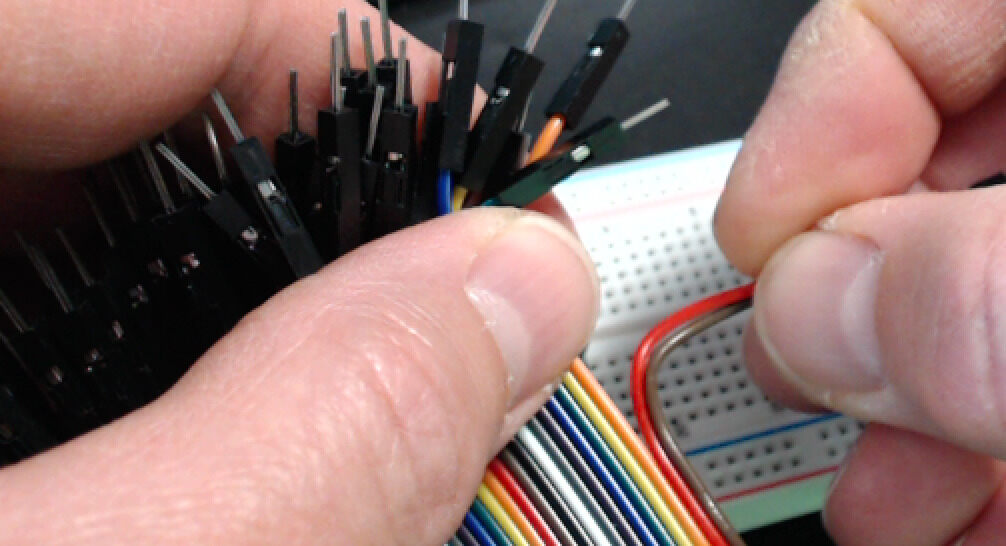
\includegraphics[width=0.4\textwidth]{direct/power/removing-two-wires}
    }
    \hfil
    \subfloat[]{
        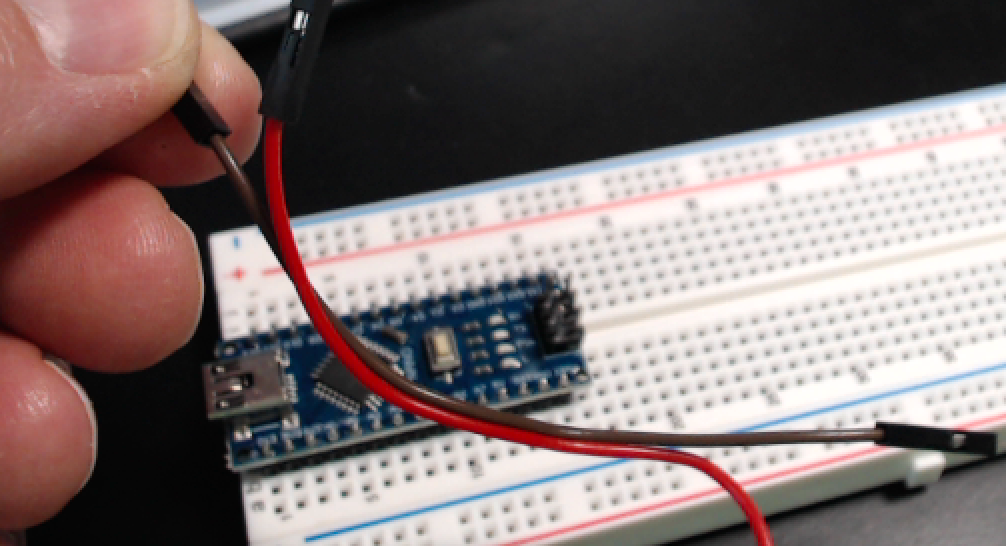
\includegraphics[width=0.4\textwidth]{direct/power/two-wires}
    }
    \caption{Removing a two-conductor cable from the 40-conductor cable.\label{fig:two-wires}}
\end{figure}

\begin{figure}
    \centering
    \subfloat[Tapping power and ground from the \developmentboard.]{
        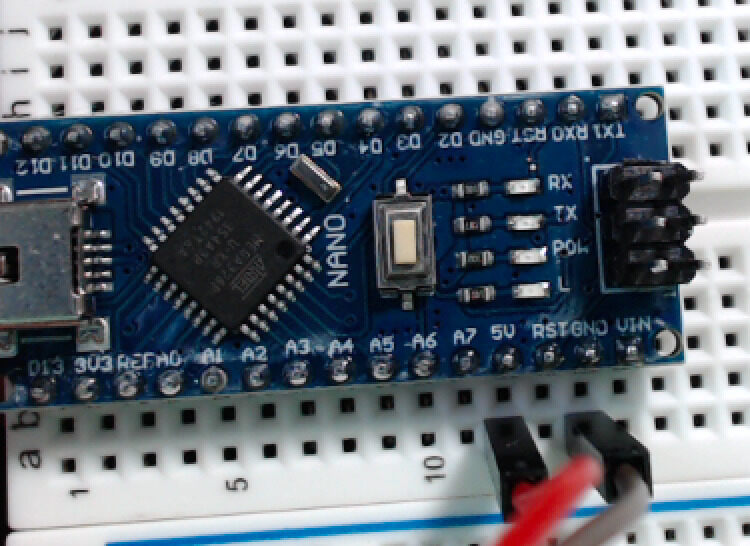
\includegraphics[width=0.27\textwidth]{direct/power/power-step-1}
        \label{fig:power-step-1}
    }
    \hfil
    \subfloat[Connecting lower power bus to power and ground.]{
        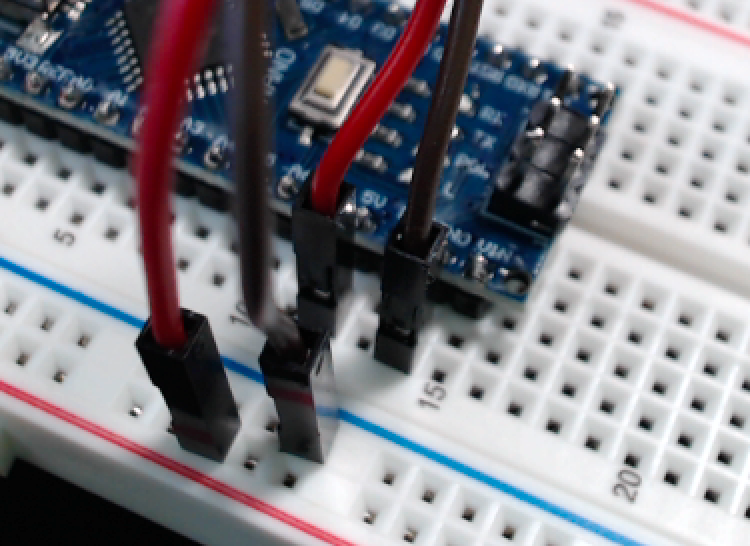
\includegraphics[width=0.27\textwidth]{direct/power/power-step-2}
        \label{fig:power-step-2}
    }
    \hfil
    \subfloat[Connecting upper and lower power busses.]{
        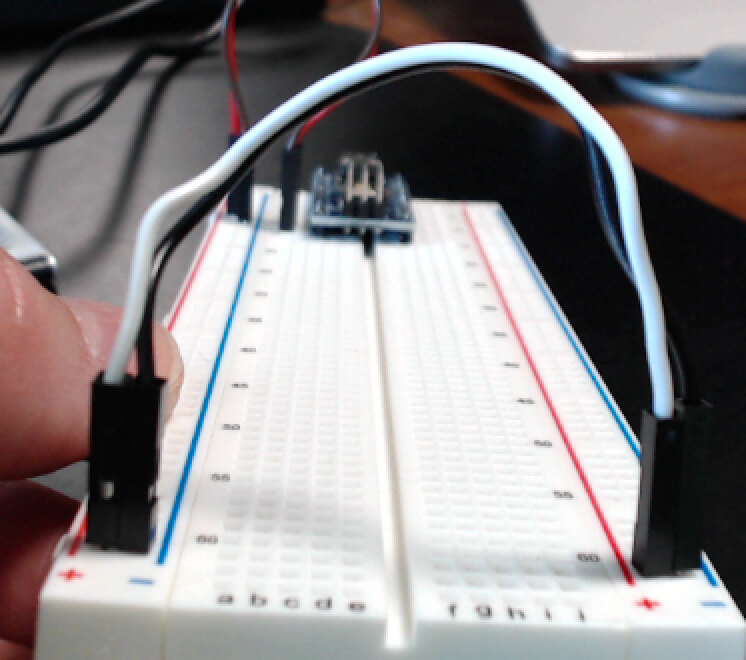
\includegraphics[width=0.27\textwidth]{direct/power/power-step-3}
        \label{fig:power-step-3}
    }
    \caption{Providing power and ground to power busses.}
\end{figure}

Peel off another 2-wire cable from the \rainbow.
Use this 2-conductor cable to connect the lower \power\ to the upper \power, and to connect the lower \ground\ to the upper \ground.
If you place this cable on the right end of the breadboard, it will be out of the way during the remaining steps;
see Figure~\ref{fig:power-step-3}. % TODO: "for now"

\checkpoint{connected the \power{}s and the \ground{}s}
